Breaking a paragraph into lines is the problem of, given a string of
words and other material with intervening spaces, breaking that string
into chunks (lines) of approximately equal length, and doing so in a
visually attractive way. Simple strategies (see the `first fit'
algorithm below) give a result that is easy to compute, but that can
be visually very unappealing. While the problem of finding globally
optimal line breaks sounds very hard --~with $n$~words there are $2^n$
ways of breaking the paragraph; also, this problem resembles the
bin-packing problem which is NP-complete~-- it can actually be solved
fairly efficiently.

\TeX's basic strategy is to calculate the badness of breaking the
lines at certain points, and to minimize the badness over the whole
paragraph.

\Level 0 {The elements of a paragraph}

\TeX's paragraph breaking algorithm is based around the concepts of
\begin{itemize}
\item Boxes: this comprises letters, formulas, \TeX\ boxes, and other
  material of a fixed with.
\item Glue: this is white space; a glue item has a natural width,
  stretchability, and shrinkability.
\item Penalties: these are items that express the desirability or
  undesirability of breaking a line at a particular point.
\end{itemize}
The same elements are also present in a vertical list; in both cases
there are some other, more rare items, that we will ignore here.

\Level 1 {Some details}

\Level 2 {Boxes}

The boxes in a paragraph are such things as words, rules, math
formulas, and actual \TeX\ \cs{box}es. A~box can not be broken: it is
completely described by its height, depth, width. Actually, looking at
words as boxes is too simplistic, since words can often be
hyphenated. This means that a word is a sequence of boxes alternating
with penalties.

\Level 2 {Penalties}

A penalty item describes the desirability or undesirability of
breaking a list at some point. Penalties can be inserted by hand (most
often as the \cs{nobreak} macro, which is equivalent to
\verb+\penalty10000+), or in a macro, or are inserted
by \TeX\ itself. An example of the latter case is the
\cs{hyphenpenalty} which discourages breaking at a hyphen in a word.

Hyphenating a word can be simulated by having a penalty of zero at the
hyphenation location. Since this usually introduces a hyphen
character, \TeX\ internally pretends that penalties can have a width
if the list is broken at that place.

The most common types of penalty are the infinite penalty that starts
a non-breaking space, and the penalty associated with breaking by
hyphenating a word. The latter kind is called a `flagged penalty', and
\TeX\ has an extra amount of demerits associated with them, for
instance to prevent two consecutive lines ending in a hyphen.

Penalties can have positive and negative values, to discourage or
encourage breaking at a specific place respectively. The values
$+\infty$ and~$-\infty$ are also allowed, corresponding to a forbidden
and forced break respectively.

\Level 2 {Glue}

A `glue' is a dimension with possible stretch and/or shrink. There are
glue denotations, such as \n{2cm plus .5cm minus .1cm}, or glue
parameters, such as \cs{leftskip} or \cs{abovedisplayskip}. The
parameters are inserted automatically by the various \TeX\ mechanisms.

Glue can be measured in points \n{pt}, centimeters \n{cm}, millimeters
\n{mm}, inches \n{in}. There is also infinite glue: \n{fil}, \n{fill},
and \n{filll}.
Presence of \TeX's infite glue
(\n{fill}) causes all other glue to be set at natural width, that is,
with zero stretch and shrink. 

If there is more than one glue item in a list, the natural widths and
the stretch and shrink amounts are added together. This means that a
list with both \n{2cm plus 1cm} and \n{2cm plus -1cm} has no stretch
since the stretch amounts add up to zero.
On the other hand, with \n{2cm plus 1cm} and \n{2cm minus 1cm} it has
both stretch and shrink.

The stretch and shrink components of glue are not treated
symmetrically. While in a pinch we can allow a line to be stretched
further than the indicated maximum, we can not allow spaces to be
shrunk to zero, or even close to that. 

\Level 2 {Stretch and shrink}

Each space can have stretch and shrink. When we consider a line, we
add up all the stretch and shrink and compute an `adjustment ratio' as
the ratio of the shortfall or excess space to the available stretch or
shrink repectively. This ratio~$r$ is negative for lines that need to be
shrunk.

A simple algorithm would be to impose a limit of~$|r|\leq\nobreak1$
(and then to minimize the number of hyphenations under that restriction),
but that might be too restrictive. Instead, \TeX\ uses a concept of
`\index{baddness!of line breaks}badness'.  The badness of a line break
is infinite if~$r<\nobreak -1$; otherwise it is cubic in the absolute
size of~$r$.

\Level 2 {Line break locations}

Here are the main (but not the only) locations where \TeX\ can decide
to break a line.
\begin{itemize}
\item At a penalty
\item At a glue, if it is preceeded by a non-discardable item,
  meaning, not a penalty or other glue
\item At a hyphen in a word
\item At a place where \TeX\ knows how to hyphenate the word. (There
  is actually a mechanism, called `discretionaries' that handles these
  last two cases.)
\end{itemize}

\Level 1 {Examples}

Here are a few examples of the things that the boxes/penalties/glue
mechanism is capable of.

\Level 1 {Centered text}

By using \cs{leftskip} and \cs{rightskip} we can get centered text.
\begin{examplewithcode}
\begin{minipage}{4cm}
\leftskip=0pt plus 1fil \rightskip=0pt plus 1fil
\parfillskip=0pt
This paragraph puts infinitely stretchable glue at 
the left and right of each line.
The effect is that the lines will be centered.
\end{minipage}
\end{examplewithcode}

The following centers only the last line. This is done by letting the
\cs{leftskip} and \cs{rightskip} cancel each other out, except on the
last line.
\begin{examplewithcode}
\begin{minipage}{5cm}
\leftskip=0pt plus 1fil \rightskip=0pt plus -1fil
\parfillskip=0pt plus 2fil
This paragraph puts infinitely stretchable glue at 
the left and right of each line, but the amounts cancel out.
The parfillskip on the last line changes that.
\end{minipage}
\end{examplewithcode}

\Level 2 {Hanging punctuation}

Hanging punctuation is a style of typesetting where punctuation that
would wind up against the right margin is actually set \emph{in} the
right margin. Optically, this makes the margin look straighter.

\begin{verbatim}
\newbox\pbox \newbox\cbox
\setbox\pbox\hbox{.} \wd\pbox=0pt
\setbox\cbox\hbox{,} \wd\cbox=0pt
\newdimen\csize \csize=\wd\cbox
\newdimen\psize \psize=\wd\pbox

\catcode`,=13 \catcode`.=13
\def,{\copy\cbox \penalty0 \hskip\csize\relax}
\def.{\copy\pbox \penalty0 \hskip\psize\relax}
\end{verbatim}

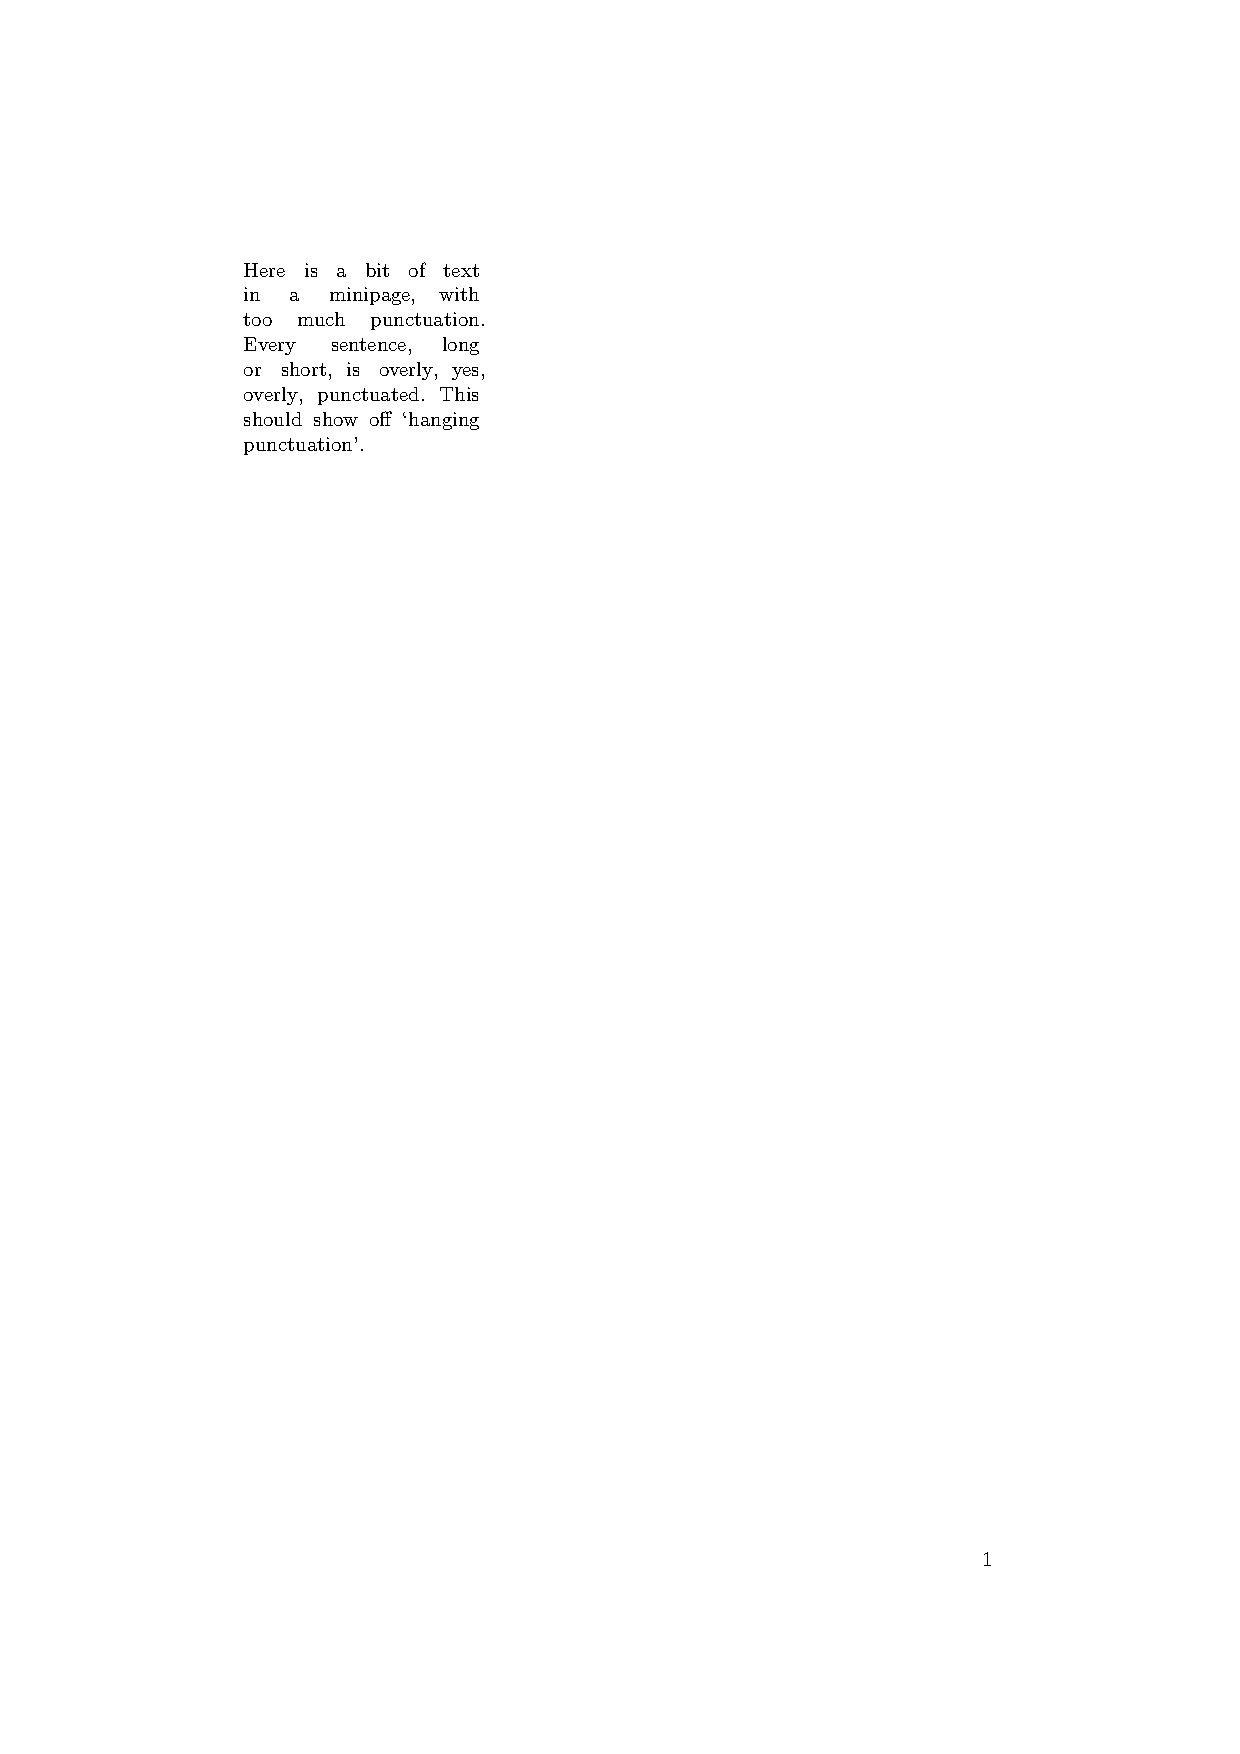
\includegraphics{hang}

\Level 2 {Mathematical Reviews}

In `Mathematical Reviews' the name of the reviewer should be separated
sufficiently from the review, but fit on the same line if space allows.

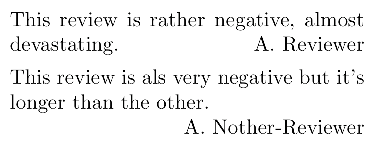
\includegraphics{mr}

We do this by having two separate infinite glues with a break in
between, and with a total natural width equal to the minimum
separation. The trick is to make sure that the second glue is not
discarded after a break, which we do by putting an invisible box at
the beginning.
\begin{verbatim}
\def\signed#1{\unskip
  \penalty10000 \hskip 40pt plus 1fill
  \penalty0
  \hbox{}\penalty10000
                \hskip 0pt plus 1fill
  \hbox{#1}%
                \par
  }
\end{verbatim}

\Level 0 {\TeX's line breaking algorithm}

\Level 1 {Elements}

\Level 2 {Glue setting and badness}
\label{sec:glue-set}

In order to make a list fit a prescribed dimension, there is a process
called `glue setting'. The natural size of the list and the desired
size are compared. Let $\rho$ be the ratio of the amount stretched
(shrunk) to the possible amount of stretch (shrink).
The exact definition is such that the ratio is positive for stretch
and negative for shrink: let $\ell$ be the desired length of the line,
$L$~the natural width, $X$~the available stretch and $Y$~the available
shrink, then
\[ \rho=\cases{
    0&$\ell=L$\cr (\ell-L)/X&(stretch:) $\ell>L$ and $X>0$\cr
    (\ell-L)/Y&(shrink:) $\ell<L$ and $Y>0$\cr
    \mathrm{undefined}&otherwise}
\]

Then the `badness' of the needed glue setting is
\[ b = \cases{
          10\,000&$\rho<1$ or undefined\cr
          \min\left\{10\,000, 100|\rho|^3\right\}&otherwise
       }
\]
Since $10\,000$ is considered infinite in glue arithmetic, this
algorithm allows glue to be stretched further than the indicated
amount, but not shrunk beyond what is available.

A list that is stretched or shrunk is put in one of the following four
categories:
\begin{itemize}
\item[\textit{tight (3)}] if it has shrunk with $b\geq 13$
\item[\textit{decent (2)}] if $b\leq12$
\item[\textit{loose (1)}] if it has stretched with $100>b\geq 13$
\item[\textit{very loose (0)}] if it has stretched with $b\geq100$
\end{itemize}
Note that $100\times(1/2)^3=12.5$, so the crossover values denote that half the
stretch or shrink is used.

Lines that differ by more than one in their classifications are called
`visually incompatible'.

\Level 2 {Demerits}

Breaking a line at a certain points gives the penalty~$p$ associated with
that point, and the badness~$b$ of the resulting stretch/shrink. These
are combined into a `demerits' figure:
\[ d=\cases{b^2+p^2&$0\leq p<10\,000$\cr b^2-p^2&$-10\,000<p<0$\cr} \]
The demerits for breaking a paragraph along a certain sequence of
break points is then the sum of the demerits of the lines, plus
\cs{adjdemerits} for every two lines that are not visually compatible
(section~\ref{sec:glue-set}), \cs{doublehyphendemerits} for pairs of
lines that end in a hyphen, and \cs{finalhyphendemerits} if the last
full line ends in a hyphen.

\TeX\ acts as if before the first line there is a line that is
`decent'; the last line will typically contain infinite glue, so all
spaces are set at natural width.

For full generality, the last line of a paragraph is handled like any
other. Filling out the line to the margin is realized by added
infinite glue plus a trailing penalty that forces a line break at the
end of the paragraph.

\Level 1 {Breaking strategies}

We will now look at a couple of line breaking strategies. The first
two will be strictly local; the third --~\TeX's algorithm~-- is able
to optimize in a more global sense.

The problem with local algorithms is that
they can not take a slightly worse solution in one line to prevent much
worse from happening later. This will for instance allow tight and
very loose lines
to occur next to each other.

\Level 2 {First fit}

The traditional algorithm for line breaking only looks at the current
line. Once a word is starting to exceed the right margin, the
following cases are investigated.
\begin{enumerate}
\item If the spaces in the line can be compressed without exceeding
  some maximum shrinkage, break after this word.
\item Otherwise, if the spaces can be stretched short of some maximum,
  break before this word.
\item Otherwise, try hyphenating this word.
\item If no hyphenation point can be found, accept a line with spaces
  stretched to whatever degree is needed to break before this word.
\end{enumerate}

If you have set text with \TeX, you will have noticed that \TeX's
solution to the last point is slightly different. It will let a word
protrude into the right margin as a visual indicator that no good
breakpoint could be found. (\TeX's tolerance to bad breaks can be
increased by setting the \cs{emergencystretch} parameter.)

This method can be called `first fit', because it will the first
option (compress), without comparing if later options (stretching)
look better. This is remedied in \TeX\ by, instead of having an
all-or-nothing it fits~/ it doesn't fit distinction, there is a
continuous scale of evaluation.

\Level 2 {Best fit}

A slight improvement on the first fit algorithm results from deciding
between the possibilities~1--3 based on badness calculations. This can
be termed `best fit', and while it may work slightly better than fit,
it is still a local decision process.

\Level 2 {Total fit}

\TeX's actual algorithm calculates the `\index{demerit!of line
  breaking}demerits' of a line break as a compound of badness, the
breakpoint penalty, plus any flagged penalties. 
It then adds together the demerits of the whole paragraph, and
minimizes this number. This makes it possible to use a slightly worse
line break early in the paragraph, to prevent a much worse one later.

\begin{594exercise}
In dynamic programming, many solutions start from a final stage and
work backwards. Why is this approach inappropriate for \TeX's
line breaking algorithm? Why would it be even less appropriate for a
page breaking algorithm?
\end{594exercise}
\begin{answer}
A forward approach is possible because the starting point is clear:
the zeroeth breakpoint is at the left margin of the first line. The
breakpoint at the beginning of the last line is not fixed in that
way. This means that we can not trivially solve the last stage.
A~forward approach to page breaking could use heuristics to flush the
memory to the output final every once in a while. A~backtracking
approach would have to store the whole document in memory before it
could start breaking.
\end{answer}

\Level 1 {Model implementation}

We will here only discuss implementations of solutions based on
dynamic programming.

The line breaking algorithm goes linearly through the items in the
horizontal list, and for each considers whether there is a valid
breakpoint after it, and with what cost. For the latter point, it
needs to know what the beginning of the line is, so there is an inner
loop over all preceeding words. This would make the running time of
the algorithm quadratic in the number of words, which is much better
than the initial estimate of~$2^n$.

However, the situation is better than that. The number of words that
can fit on a line is limited by what can fit when all spaces are
sqeezed to zero. The easiest way to implement this is by maintaining
an `active list' of possible words to begin the line with. A~word can
be removed from the active list if the material from it to the current
word does not fit: if it does not fit now, it will certainly not fit
when the next word is considered.

This is then the main program; we will mainly vary the function that
computes the breakpoint cost.
\begin{verbatim}
active = [0]
nwords = len(paragraph)
for w in range(1,nwords):
    # compute the cost of breaking after word w
    for a in active:
        line = paragraph[a:w+1]
        ratio = compute_ratio(line)
        if w==nwords-1 and ratio>0:
            ratio = 0 # last line will be set perfect
        print "..line=",line,"; ratio=",ratio
        if ratio<-1:
            active.remove(a)
            print "active point",a,"removed"
        else:
            update_cost(a,w,ratio)
    report_cost(w)
    active.append(w)
    print
\end{verbatim}
The only thing different between various strategies is how the cost of
a line break is computed by \n{update_cost(a,w,ratio)}.

\begin{594exercise}
Not every word should be added to the active list. For instance, for
any realistic line length, the second word in the paragraph will not
have a valid breakpoint after it, so we need not consider it.  Take
the model implementation and add this modification. Measure the
improvement in running time, for instance by counting the number of
calls to some inner routine.  Give a theoretical argument for how this
reduces the complexity of the algorithm.
\end{594exercise}
\begin{answer}
Assume that at the end of the first line there will be two
breakpoints, one for a stretched and one for a shrunk line. At the end
of the second line there will be four possibilities, of which two
(stretch/shrink and shrink/stretch) are the same, giving three
breakpoints. Four feasible breakpoints at the end of the third line,
et cetera.

For short paragraphs this means that the cost will be roughly
quadratic in the number of lines of the paragraph.

After a number of lines, the breakpoints will merge: a certain breakpoint
will be feasible from $k$ stretched lines and from $k+1$ shrunk
ones. From that point on, every word introduces a feasible breakpoint,
so the cost is linear in the number of words to the end of the
paragraph and the number of words per line.
\end{answer}

\Level 2 {First fit implementation}

Since at first we are looking only locally, for each breakpoint we
only keep track of the cost and the previous breakpoint that the cost
was computed from.  Here we set up the data structure
\n{cost}. Element \n{cost[w]} describes the cost of breaking after
word~\n{w}; the \n{'from'} component is the number of the first word
of the line.
\begin{verbatim}
def init_costs():
    global cost
    cost = len(paragraph)*[0]
    for i in range(len(paragraph)):
        cost[i] = {'cost':0, 'from':0}
    cost[0] = {'cost':10000, 'from':-1}
\end{verbatim}

The essential function is the cost computation. In first fit we accept
any stretch or shrink that is~$|\rho|<\nobreak1$.
\begin{verbatim}
def update_cost(a,w,ratio):
    global cost
    if a>0 and cost[a-1]['cost']<10000:
        if ratio<=1 and ratio>=-1:
            to_here = abs(ratio)
        else: to_here = 10000
        if cost[w]['cost']==0 or to_here<cost[w]['cost']:
            cost[w]['cost'] = to_here; cost[w]['from'] = a-1
\end{verbatim}
(The first test serves to make sure that the previous point being
considered is in fact a valid breakpoint.)

Here is the remaining function that constructs the chain of breakpoints:
\begin{verbatim}
def final_report():
    global cost,nwords,paragraph
    print "Can break this paragraph at cost",\
        cost[nwords-1]['cost']
    cur = len(paragraph)-1; broken = []
    while cur!=-1:
        prev = cost[cur]['from']
        line = paragraph[prev+1:cur+1]
        broken.insert(0,line)
        cur = prev;
    set_paragraph(broken)
\end{verbatim}

A small example text, faked in monospace:
\begin{footnotesize}
\begin{verbatim}
You may  never  have  thought  of  it,  but  fonts  (better:   -0.111111111111
typefaces) usually have a mathematical  definition  somehow.   -0.666666666667
If   a   font   is   given   as   bitmap,   this   is  often   0.888888888889
a  result  originating  from  a  more  compact  description.   0.0
Imagine the situation that you have bitmaps at  300dpi,  and   -0.777777777778
you   buy   a  600dpi  printer.  It  wouldn't  look  pretty.   0.25
There   is   then   a   need   for  a  mathematical  way  of   0.555555555556
describing  arbitrary  shapes.  These  shapes  can  also  be   0.0
three-dimensional; in fact,  a~lot  of  the  mathematics  in   -0.285714285714
this  chapter  was  developed  by  a  car  manufacturer  for   0.0
modeling   car   body  shapes.  But  let  us  for  now  only   0.222222222222
look   in  two  dimensions,  which  means  that  the  curves   0.125
are  lines,  rather  than  planes.
\end{verbatim}
\end{footnotesize}
We see ugly stretched break in line~3, especially after the compressed
line~2. However, both of them fit the test.
\begin{problem}
This is not really first fit. Line~3 should have contained the~`a',
because it does not extend into the margin.
\end{problem}

It is in fact simple to turn this into a dynamic programming solution
that considers a global minimum:
\begin{verbatim}
def update_cost(a,w,ratio):
    global cost
    if ratio<=1 and ratio>=-1:
        to_here = abs(ratio)
    else: to_here = 10000
    if a>0:
        from_there = cost[a-1]['cost']
        to_here = to_here+from_there
    else: from_there = 0
    if cost[w]['cost']==0 or to_here<cost[w]['cost']:
        cost[w]['cost'] = to_here; cost[w]['from'] = a-1
\end{verbatim}

\Level 2 {Best fit}

In the best fit strategy, we compute badness from the stretch/shrink ratio.
This involves only a slight change in the cost computation function:
\begin{verbatim}
def update_cost(a,w,ratio):
    global cost
    to_here = 100*abs(ratio)**2
    if a>0:
        from_there = cost[a-1]['cost']
        to_here = to_here+from_there
    else: from_there = 0
    if cost[w]['cost']==0 or to_here<cost[w]['cost']:
        cost[w]['cost'] = to_here; cost[w]['from'] = a-1
\end{verbatim}
The same text:
\begin{footnotesize}
\begin{verbatim}
You may  never  have  thought  of  it,  but  fonts  (better:   -0.111111111111
typefaces) usually have a mathematical  definition  somehow.   -0.666666666667
If   a   font   is   given   as  bitmap,  this  is  often  a   0.5
result   originating   from   a  more  compact  description.   0.5
Imagine the situation that you have bitmaps at  300dpi,  and   -0.777777777778
you   buy   a  600dpi  printer.  It  wouldn't  look  pretty.   0.25
There   is   then   a   need   for  a  mathematical  way  of   0.555555555556
describing  arbitrary  shapes.  These  shapes  can  also  be   0.0
three-dimensional; in fact,  a~lot  of  the  mathematics  in   -0.285714285714
this  chapter  was  developed  by  a  car  manufacturer  for   0.0
modeling   car   body  shapes.  But  let  us  for  now  only   0.222222222222
look   in  two  dimensions,  which  means  that  the  curves   0.125
are  lines,  rather  than  planes.
\end{verbatim}
\end{footnotesize}
While there are no lines stretched with $\rho>$, the quadratic
function has improved the break in line~3.

\Level 2 {Total fit}

For the algorithm that \TeX\ uses, we have to distinguish between
lines that are tight, decent, loose. This makes our datastructure more
complicated:
\begin{problem}
Where is the fourth category?
\end{problem}
\begin{verbatim}
def init_costs():
    global cost
    nul = [0,0,0]
    cost = len(paragraph)*[ 0 ]
    for i in range(len(paragraph)):
        cost[i] = nul[:]
        for j in range(3):
            cost[i][j] = {'cost':10000, 'from':-2}
    for j in range(3):
        cost[0][j] = {'cost':10000, 'from':-1}
\end{verbatim}
An element \n{cost[i]} is now an array of three possible breakpoints,
one in each of the classifications. An actual breakpoint is now in
\n{cost[word][type]['from']} and \n{cost[word][type]['cost']}.

The cost computation becomes more complicated:
\begin{verbatim}
def minimum_cost_and_type(w):
    global cost
    c = 10000; t = 0
    for type in range(3):
        nc = cost[w][type]['cost']
        if nc<c:
            c = nc; t = type
    return [c,t]
def update_cost(a,w,ratio):
    global cost
    type = stretch_type(ratio)
    to_here = 100*abs(ratio)**2
    if a>0:
        [from_there,from_type] = minimum_cost_and_type(a-1)
        to_here += from_there
    else: from_there = 0
    if cost[w][type]['cost']==0 or\
       to_here<cost[w][type]['cost']:
        cost[w][type]['cost'] = to_here;
        cost[w][type]['from'] = a-1
\end{verbatim}
\begin{594exercise}
The total fit code does not yet contain the equivalent of \TeX's
\cs{adjdemerits}. Add that.
\end{594exercise}

Let us look at the same test text again:
\begin{footnotesize}
\begin{verbatim}
You may  never  have  thought  of  it,  but  fonts  (better:   -0.111111111111
typefaces)   usually   have   a   mathematical   definition   1.2
somehow. If a font is given  as  bitmap,  this  is  often  a   -0.454545454545
result   originating   from   a  more  compact  description.   0.5
Imagine   the   situation   that   you   have   bitmaps   at   1.0
300dpi, and you buy  a  600dpi  printer.  It  wouldn't  look   -0.333333333333
pretty. There is then a  need  for  a  mathematical  way  of   -0.4
describing  arbitrary  shapes.  These  shapes  can  also  be   0.0
three-dimensional; in fact,  a~lot  of  the  mathematics  in   -0.285714285714
this  chapter  was  developed  by  a  car  manufacturer  for   0.0
modeling   car   body  shapes.  But  let  us  for  now  only   0.222222222222
look   in  two  dimensions,  which  means  that  the  curves   0.125
are  lines,  rather  than  planes.
\end{verbatim}
\end{footnotesize}
In this output, line~2 is stretched further than before, to prevent
lower badnesses later.

\begin{594exercise}
Add the functionality for hanging indentation to this code.
\end{594exercise}
\begin{594exercise}
(bonus point exercise)
\TeX\ has the possibility of forcing a paragraph to be a line longer
or shorter than optimal. Implement that.
\end{594exercise}

\Level 2 {Utility parts}

File header: we read a text and store it.
\begin{verbatim}
#! /usr/bin/env python

import sys

max_line_length = 60

paragraph = []
while 1:
    try:
        a = raw_input()
        paragraph.extend(a.split())
    except (EOFError):
        break
\end{verbatim}

In order to fake stretch and shrink with a monospace font, we let a
`space' be two spaces by default.
\begin{verbatim}
def line_length(words):
    l = 2*(len(words)-1)
    for w in words:
        l += len(w)
    return l
#
# ratio = -1 : shrink each double space to one
# ratio = 1 : stretch each double space to three
#
def compute_ratio(line):
    spaces = len(line)-1
    need = 1.*(max_line_length-line_length(line))
    #print "ratio:",need,spaces
    if spaces==0: return 10000
    else: return need/spaces
\end{verbatim}
Output formatting with this idea:
\begin{verbatim}
def set_paragraph(para):
    for l in range(len(para)-1):
        line = para[l]
        set_line(line)
    set_last_line(para[len(para)-1])
def set_line(line):
    shortfall = max_line_length-line_length(line)
    for w in range(len(line)-1):
        sys.stdout.write(line[w])
        if shortfall>0:
            sys.stdout.write('   '); shortfall = shortfall-1
        elif shortfall<0:
            sys.stdout.write(' '); shortfall = shortfall+1
        else:
            sys.stdout.write('  ')
    sys.stdout.write(line[len(line)-1])
    print "  ",compute_ratio(line)
def set_last_line(line):
    for w in range(len(line)-1):
        sys.stdout.write(line[w])
        sys.stdout.write('  ')
    sys.stdout.write(line[len(line)-1])
    print
\end{verbatim}
